\documentclass[10pt]{beamer}
\usepackage[T2A]{fontenc}       %поддержка кириллицы
\usepackage[utf8]{inputenc}
\usepackage{lmodern}
\usepackage{scrextend}
\changefontsizes{16pt}
\usepackage{listings}
\usepackage{xcolor}
\graphicspath{{./images/}}
\usetheme{default}
\usecolortheme{crane}
\usefonttheme{structurebold}
\usefonttheme[onlymath]{serif}
\setbeamercovered{transparent}
\definecolor{name}{rgb}{0.5,0.5,0.5}
\begin{frame}{PHP}
  \begin{center}
    \begin{itemize}
      \item Interpretation
      \item Dynamic typing
      \item Garbage collector
      \item Procedure \& OOP
    \end{itemize}
  \end{center}
\end{frame}
\definecolor{mygray}{rgb}{0.5,0.5,0.5}
\definecolor{mymauve}{rgb}{0.58,0,0.82}
\definecolor{dkgreen}{rgb}{0,.6,0}
\definecolor{dkblue}{rgb}{0,0,.6}
\definecolor{dkyellow}{cmyk}{0,0,.8,.3}

\lstdefinestyle{htmlCode} {
   language=html,
   basicstyle=\tiny\ttfamily,
   keywordstyle=\ttfamily,
   commentstyle=\color{gray}\ttfamily,
   tabsize=1,
   frame=none,
   columns=fullflexible,
   escapechar=| % Escape to LaTeX between |...|
}
\begin{frame}{CSS}
CSS (Cascading Style Sheets) — формальный язык описания внешнего вида документа, написанного с использованием языка разметки.
\end{frame}
\begin{frame}[fragile]
 	\frametitle{CSS}
    \lstinputlisting[style=cssCode, linerange={9-11}, basicstyle=\footnotesize]{sources/code/html/class.css}
\end{frame}

% Set custom colors
\definecolor{code}{gray}{0}
\definecolor{canvas}{gray}{0.96}
\definecolor{comment}{rgb}{0, 0.456, 0}
\definecolor{keyword}{rgb}{0.5, 0, 0.5}

% JavaScript is not part of the listings package...
% but thankfully this page shows how to add it:
% http://lenaherrmann.net/2010/05/20/javascript-syntax-highlighting-in-the-latex-listings-package

\lstdefinelanguage{javascript}{
  keywords={typeof, new, true, false, catch, function, return, null, catch, switch, var, if, for, in, while, do, else, case, break},
  ndkeywords={class, export, boolean, throw, implements, import, this},
  sensitive=false,
  comment=[l]{//},
  morecomment=[s][\color{blue}\ttfamily]{/*}{*/},
  morestring=[b]',
  morestring=[b]"
}

% Parameters for formatting code (optional, affects all code listings)
\lstset{
  backgroundcolor=\color{canvas},
  basicstyle=\ttfamily\small\color{code},
  commentstyle=\color{comment},
  identifierstyle=\color{black},
  keywordstyle=\color{keyword}\bfseries,
  ndkeywordstyle=\color{keyword}\bfseries,
  stringstyle=\color{blue}\ttfamily
}

\lstdefinestyle{jsCode} {
   language=javascript,
   basicstyle=\tiny\ttfamily,
   keywordstyle=\ttfamily,
   commentstyle=\color{gray}\ttfamily,
   tabsize=1,
   frame=none,
   columns=fullflexible,
   escapechar=| % Escape to LaTeX between |...|
}
\definecolor{mygray}{rgb}{0.5,0.5,0.5}
\definecolor{mymauve}{rgb}{0.58,0,0.82}
\definecolor{dkgreen}{rgb}{0,.6,0}
\definecolor{dkblue}{rgb}{0,0,.6}
\definecolor{dkyellow}{cmyk}{0,0,.8,.3}

\lstdefinestyle{pascalCode} {
   language=pascal,
   basicstyle=\tiny\ttfamily,
   keywordstyle=\ttfamily,
   commentstyle=\color{gray}\ttfamily,
   tabsize=1,
   frame=none,
   columns=fullflexible,
   escapechar=| % Escape to LaTeX between |...|
}
\newcommand{\includecode}[2][c]{\lstinputlisting[caption=#2, escapechar=, style=custom#1]{#2}}


\title[Web]{Web программирование}
\subtitle[Web servers]{Web servers}
\author[Родионов И.Н.]{Игорь Родионов}
\institute[ОмГТУ ИВТ]{Омский Государственный Технический Университет\\
	{\tiny кафедра Информатики и вычислительной техники}\\
}
\date[2014]{ОмГТУ, 2014.}

\begin{document}
\begin{frame}[plain]
\maketitle
\end{frame}

\begin{frame}{Main Rule}
  \LARGE
  \begin{center}
    НЕ ДОВЕРЯЙТЕ ВХОДНЫМ ДАННЫМ
  \end{center}
\end{frame}
\begin{frame}{Web Server - Архитектура}
  \begin{center}
    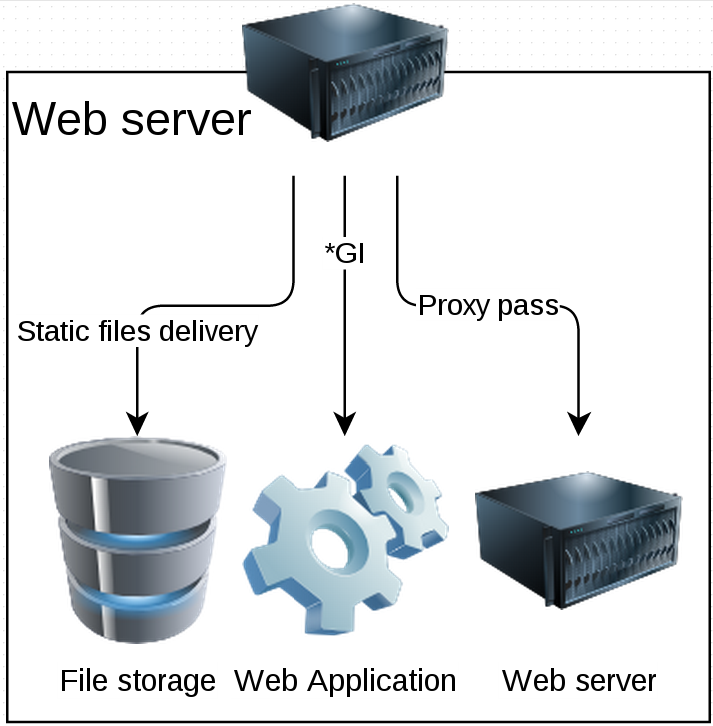
\includegraphics[height=7cm,keepaspectratio]{sources/images/Web_Server_architecture.png}
  \end{center}
\end{frame}
\begin{frame}{Web Server - Proxy}
  \begin{center}
    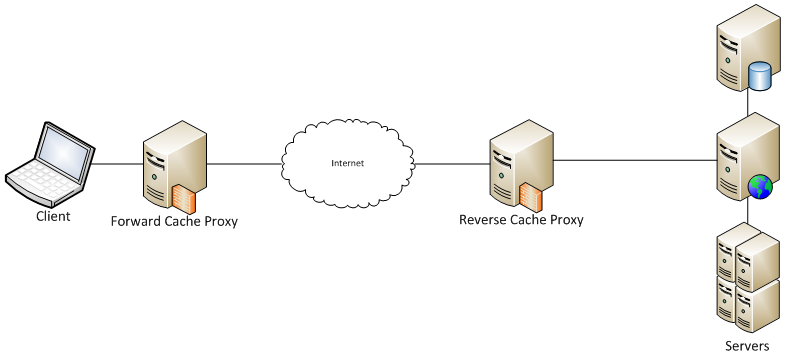
\includegraphics[width=\textwidth,keepaspectratio]{sources/images/proxy_cache_topology.png}
  \end{center}
\end{frame}
\begin{frame}[fragile]{Web Server - CGI}
  \begin{center}
    Сommon Gateway Interface — стандарт интерфейса, используемого для связи внешней программы с веб-сервером.
    Интерфейс разработан чтобы работать со стандартными устройствами ввода-вывода.
  \end{center}
\end{frame}

\begin{frame}[fragile]{Web Server - CGI}
  \begin{center}
    \lstinputlisting[style=pascalCode, basicstyle=\footnotesize]{sources/code/webservers/pascal_cgi.pascal}
  \end{center}
\end{frame}
\begin{frame}{Questions}
 \begin{center}
    {\LARGE Вопросы?}
 \end{center}
\end{frame}
\begin{frame}[fragile]{Concurrency}
  \begin{center}
    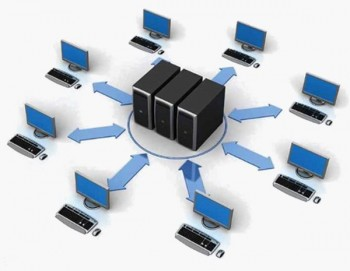
\includegraphics[height=7cm,keepaspectratio]{sources/images/socket-api-3-350x271.jpg}
  \end{center}
\end{frame}



\begin{frame}[fragile]{Concurrency}
  \begin{center}
    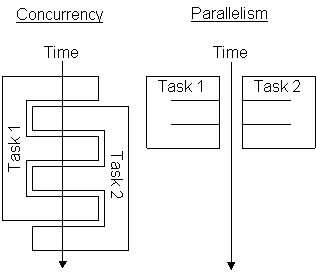
\includegraphics[height=7cm,keepaspectratio]{sources/images/concurrency-100158287-orig.png}
  \end{center}
\end{frame}

\begin{frame}[fragile]{Concurrency}
  \begin{center}
    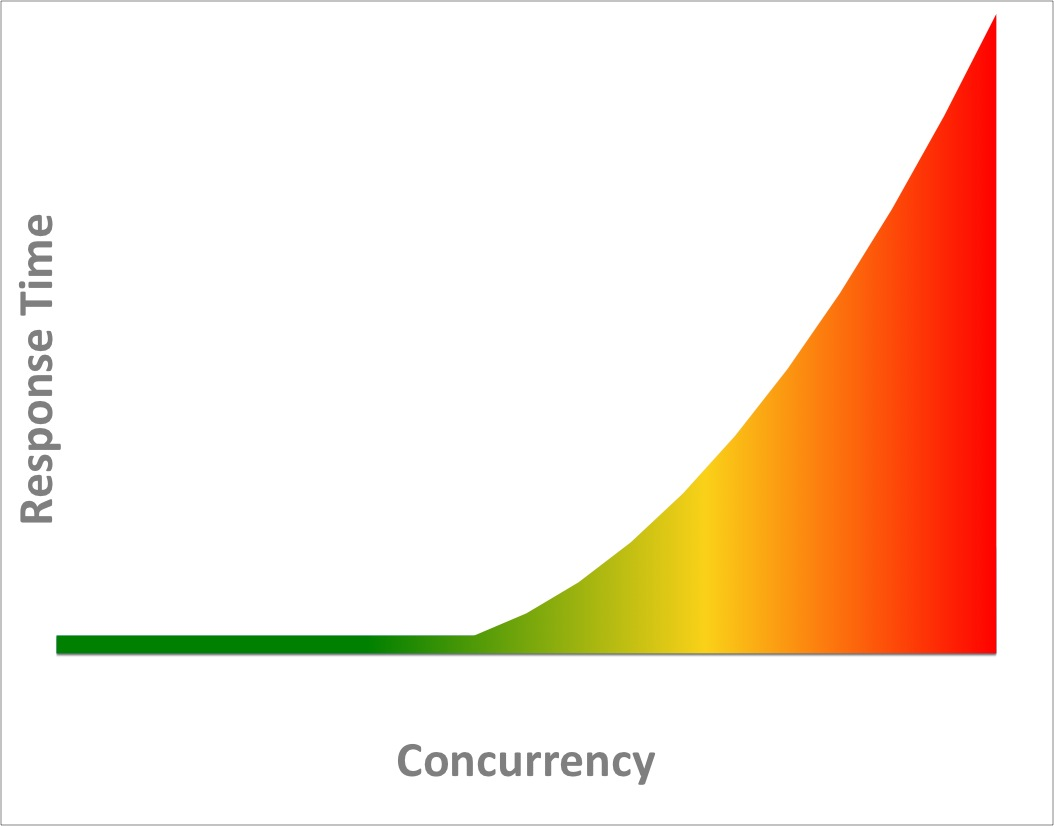
\includegraphics[height=7cm,keepaspectratio]{sources/images/response_time.jpg}
  \end{center}
\end{frame}


\begin{frame}[fragile]{Concurrency}
    \begin{columns}[t] % contents are top vertically aligned
         \begin{column}[T]{5cm} % each column can also be its own environment
            \begin{center}
              
\includegraphics[width=\textwidth,keepaspectratio]{sources/images/etot-nelovkiy-moment_9027667_big_.png}
            \end{center}
         \end{column}
         \begin{column}[T]{5cm} % alternative top-align that's better for graphics
            \begin{center}
            Этот неловкий момент, когда для объяснения материала курса, надо рассказать другой курс.
            \end{center}
         \end{column}
     \end{columns}
\end{frame}

\begin{frame}[fragile]{Concurrency}
    \begin{columns}[t] % contents are top vertically aligned
         \begin{column}[T]{5cm} % each column can also be its own environment
            \begin{center}
              
\includegraphics[width=\textwidth,keepaspectratio]{sources/images/etot-nelovkiy-moment_9027667_big_.png}
            \end{center}
         \end{column}
         \begin{column}[T]{5cm} % alternative top-align that's better for graphics
            \begin{center}
            Этот неловкий момент, когда для объяснения материала курса, надо рассказать другой курс.
            \end{center}
         \end{column}
     \end{columns}
\end{frame}

\begin{frame}{Process VS Thread}
  \begin{center}
    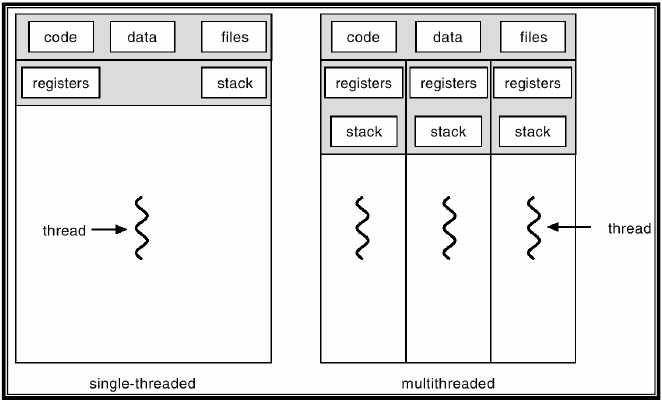
\includegraphics[width=\textwidth,keepaspectratio]{sources/images/threadmodel.png}
  \end{center}
\end{frame}

\begin{frame}{Process}
  \begin{center}
    \begin{itemize}
      \item Parent
      \item Child
      \item Zombie
      \end{itemize}
  \end{center}
\end{frame}

\begin{frame}{Process VS Thread}
  \begin{center}
    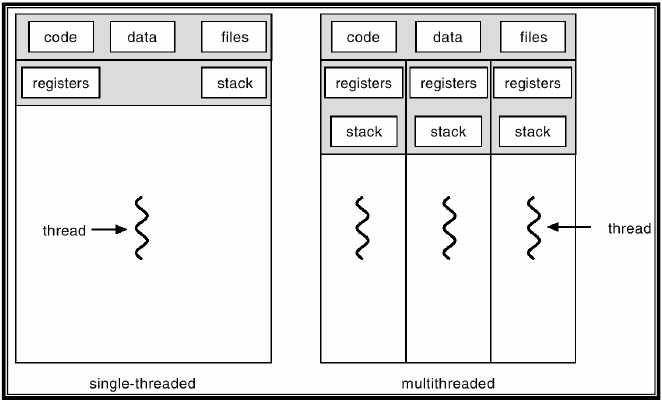
\includegraphics[width=\textwidth,keepaspectratio]{sources/images/threadmodel.png}
  \end{center}
\end{frame}

\begin{frame}{Syncronization}
  \begin{center}
    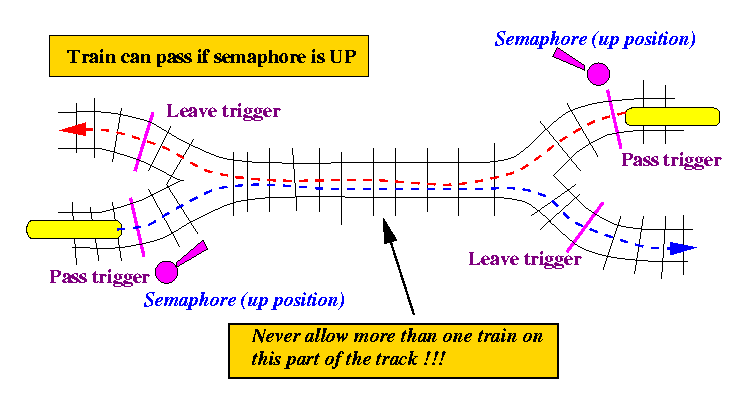
\includegraphics[width=\textwidth,keepaspectratio]{sources/images/semaphore.png}
  \end{center}
\end{frame}

\begin{frame}{Syncronization}
  \begin{center}
    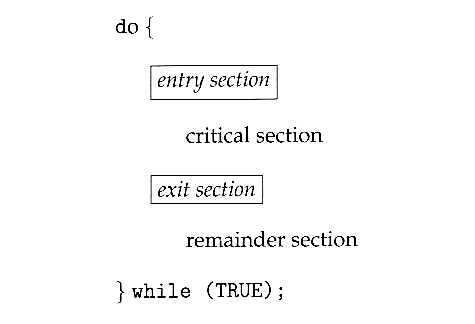
\includegraphics[width=\textwidth,keepaspectratio]{sources/images/5_01_CriticalSection.jpg}
  \end{center}
\end{frame}

\begin{frame}{Questions}
 \begin{center}
    {\LARGE Вопросы?}
 \end{center}
\end{frame}
\begin{frame}{Process communication and sharing}
  \begin{center}
    \begin{itemize}
      \item File
      \item Signals
      \item Shared memory
      \item Pipe
      \item Unix socket
      \item Socket
      \end{itemize}
  \end{center}
\end{frame}
\begin{frame}{Questions}
 \begin{center}
    {\LARGE Вопросы?}
 \end{center}
\end{frame}
\begin{frame}[fragile]{Concurrency}
  \begin{center}
    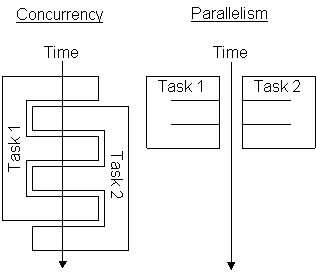
\includegraphics[height=7cm,keepaspectratio]{sources/images/concurrency-100158287-orig.png}
  \end{center}
\end{frame}

\begin{frame}{Process based architecture}
  \begin{center}
    Process\textbackslash Thread per Request
  \end{center}
\end{frame}
\begin{frame}{Apache architecture}
  \begin{center}
    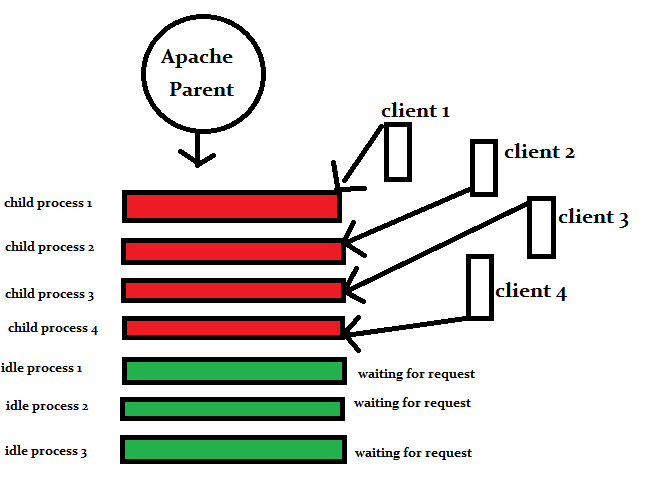
\includegraphics[height=7cm,keepaspectratio]{sources/images/prefork_model.png}
  \end{center}
\end{frame}
\begin{frame}{Apache architecture}
  \begin{center}
    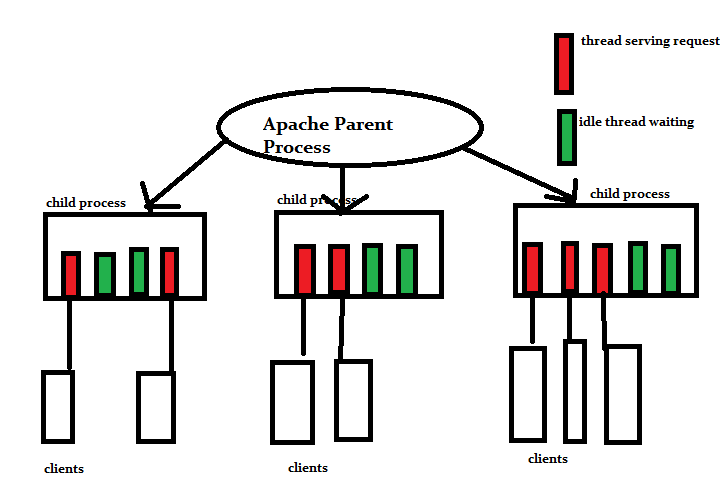
\includegraphics[height=7cm,keepaspectratio]{sources/images/apache_worker.png}
  \end{center}
\end{frame}
\begin{frame}{Questions}
 \begin{center}
    {\LARGE Вопросы?}
 \end{center}
\end{frame}
\begin{frame}{Process based}
  \begin{center}
    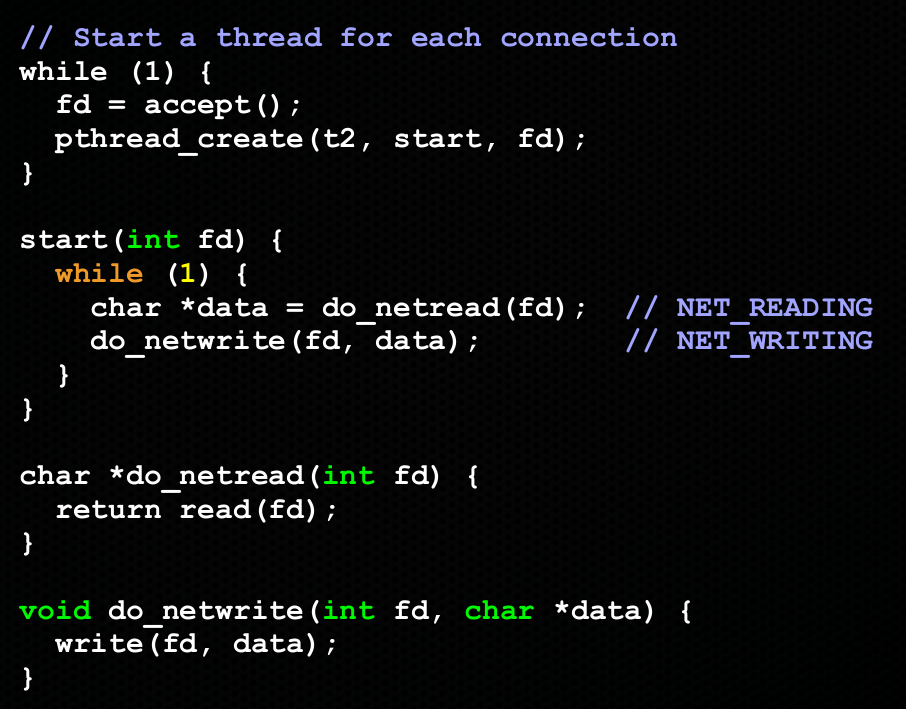
\includegraphics[height=7cm,keepaspectratio]{sources/images/process-based.png}
  \end{center}
\end{frame}
\begin{frame}{Non blocking IO}
  \begin{center}
    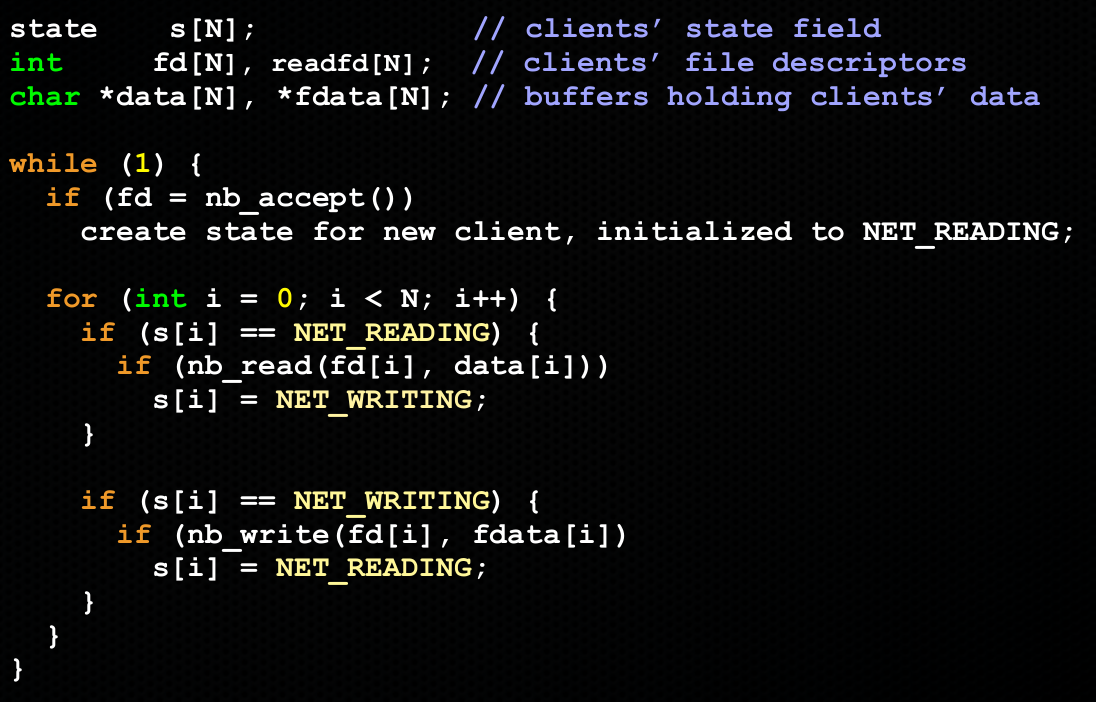
\includegraphics[width=\textwidth,keepaspectratio]{sources/images/noblocking_io.png}
  \end{center}
\end{frame}
\begin{frame}{Event based architecture}
  \begin{center}
    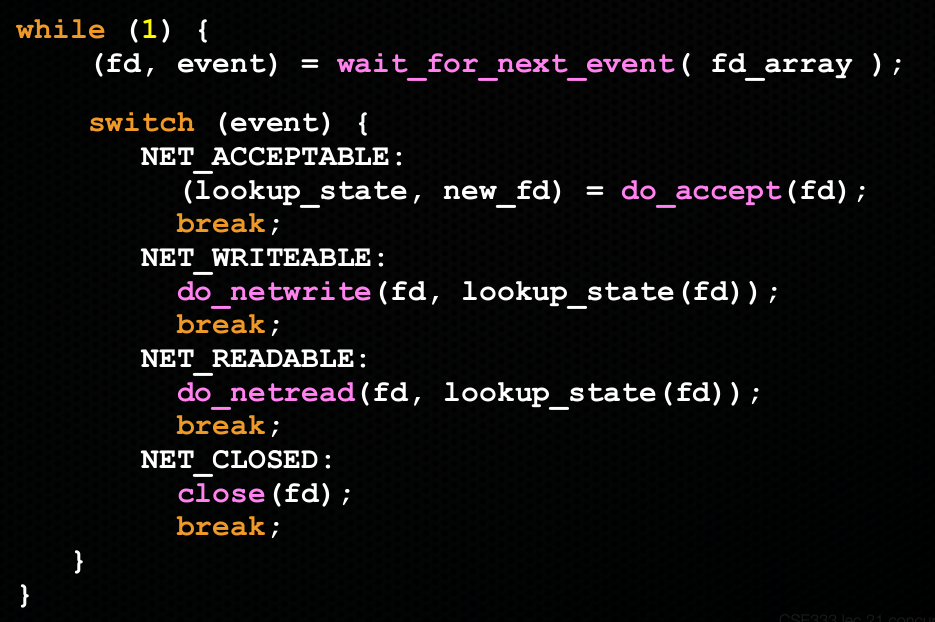
\includegraphics[width=\textwidth,keepaspectratio]{sources/images/event_based.png}
  \end{center}
\end{frame}

\begin{frame}{Event based architecture}
  \begin{center}
    \begin{itemize}
      \item Select/Poll - O(n)
      \item Epoll/Kqueue - O(1)
    \end{itemize}
  \end{center}
\end{frame}
\begin{frame}{Nginx architecture}
  \begin{center}
    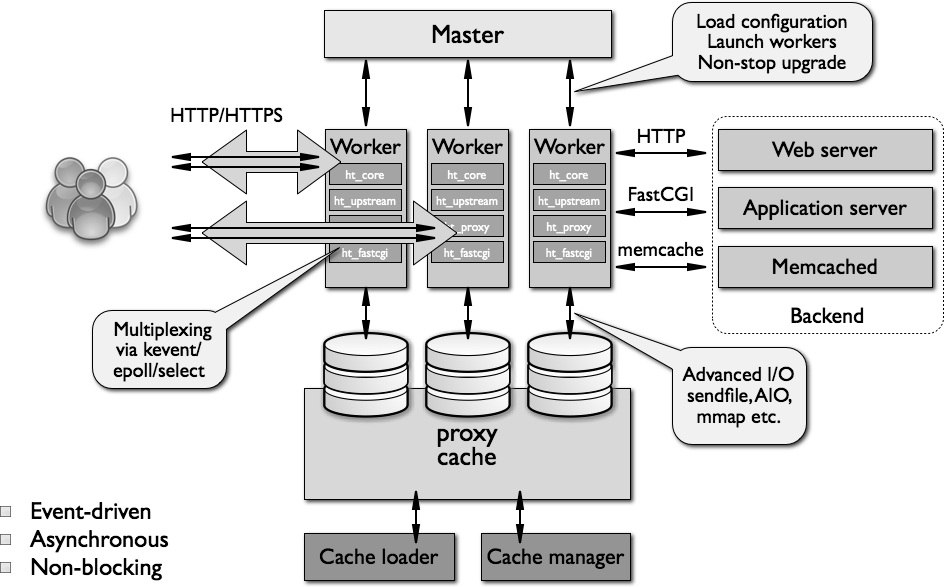
\includegraphics[width=\textwidth,keepaspectratio]{sources/images/nginx_architecture.png}
  \end{center}
\end{frame}

\begin{frame}{Apache VS Nginx}
  \begin{center}
    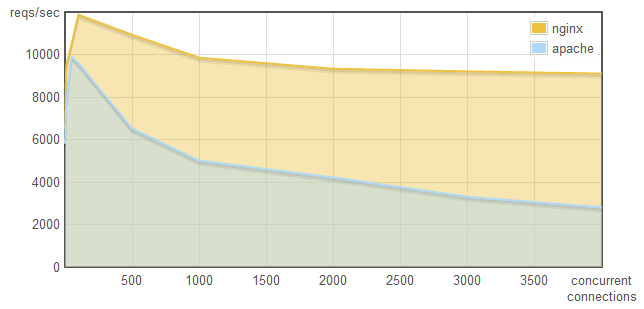
\includegraphics[width=\textwidth,keepaspectratio]{sources/images/nginx-apache-reqs-sec.png}
  \end{center}
\end{frame}
\begin{frame}{Questions}
 \begin{center}
    {\LARGE Вопросы?}
 \end{center}
\end{frame}
\begin{frame}[fragile]{Web Server - CGI}
  \begin{center}
    \lstinputlisting[style=pascalCode, basicstyle=\footnotesize]{sources/code/webservers/pascal_cgi.pascal}
  \end{center}
\end{frame}
\begin{frame}[fragile]{Web Server - FastCGI}
  \begin{center}
    Fast Сommon Gateway Interface — дальнейшее развитие технологии CGI. По сравнению с CGI является более производительным и безопасным.
  \end{center}
  \begin{center}
    \begin{itemize}
      \item Deamon
      \item TCP\textbackslash Unix Socket
      \item Separeted user
      \item Separeted server
    \end{itemize}
  \end{center}
\end{frame}
\begin{frame}{Questions}
 \begin{center}
    {\LARGE Вопросы?}
 \end{center}
\end{frame}
\begin{frame}{Load balancing}
  \begin{center}
    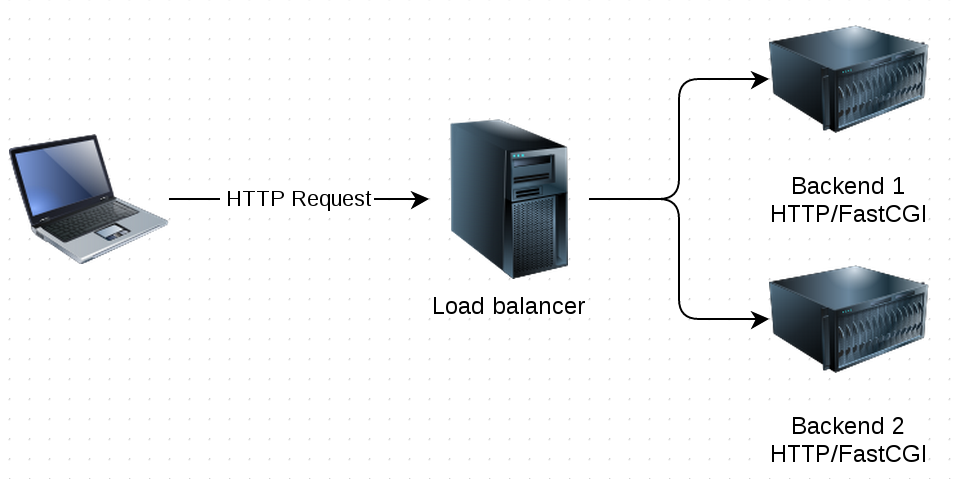
\includegraphics[width=\textwidth,keepaspectratio]{sources/images/lb.png}
  \end{center}
\end{frame}

\begin{frame}{Load balancing}
  \begin{center}
    \begin{itemize}
      \item Round-robin
      \item Weight round-robin
      \item IP sticky
      \item Sesion sticky
      \item Region sticky
    \end{itemize}
  \end{center}
\end{frame}

\begin{frame}{Session share}
  \begin{center}
    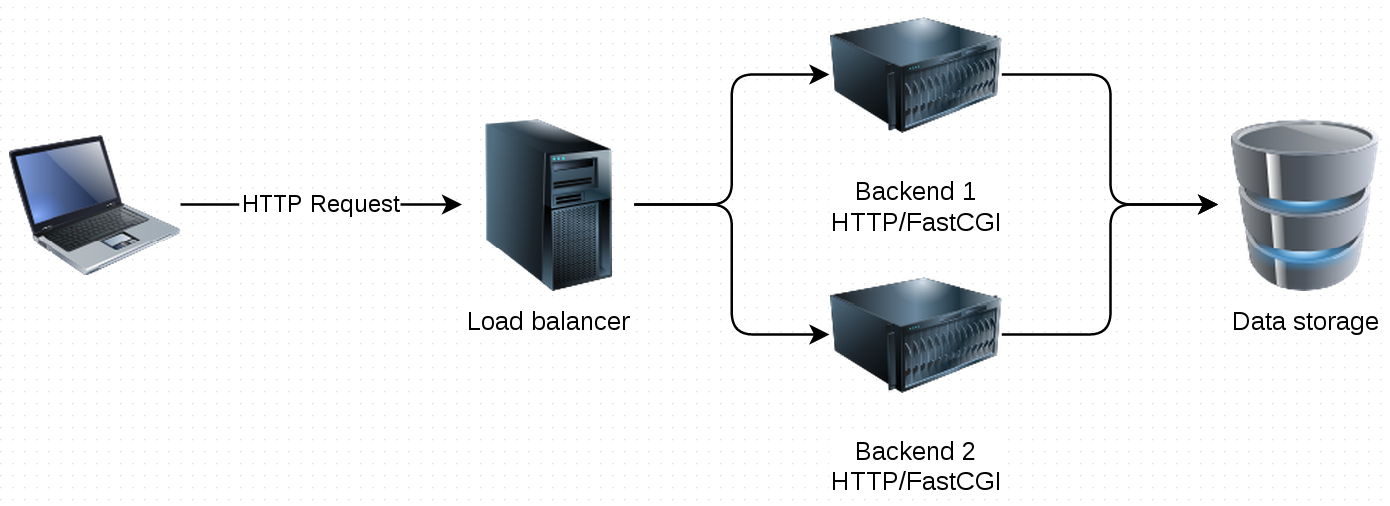
\includegraphics[width=\textwidth,keepaspectratio]{sources/images/lb_session_share.png}
  \end{center}
\end{frame}
\begin{frame}{Session sticky}
  \begin{center}
    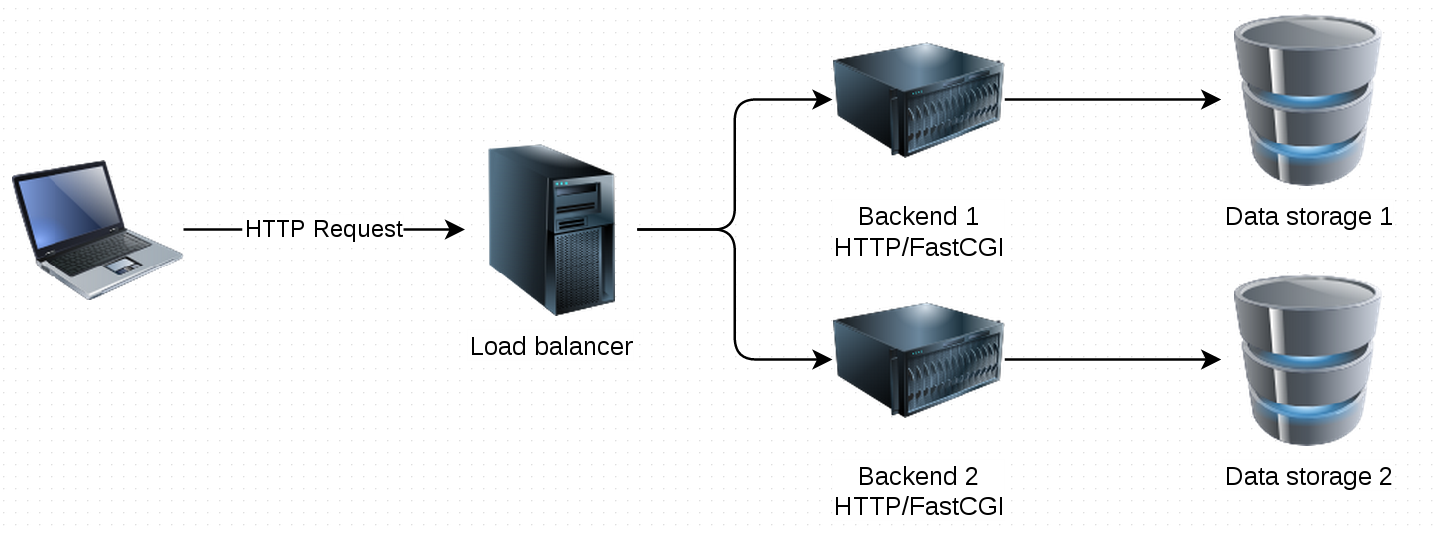
\includegraphics[width=\textwidth,keepaspectratio]{sources/images/lb_session_sticky.png}
  \end{center}
\end{frame}
\begin{frame}{Questions}
 \begin{center}
    {\LARGE Вопросы?}
 \end{center}
\end{frame}
\end{document}

